\documentclass[12pt,]{article}
\usepackage{lmodern}
\usepackage{amssymb,amsmath}
\usepackage{ifxetex,ifluatex}
\usepackage{fixltx2e} % provides \textsubscript
\ifnum 0\ifxetex 1\fi\ifluatex 1\fi=0 % if pdftex
  \usepackage[T1]{fontenc}
  \usepackage[utf8]{inputenc}
\else % if luatex or xelatex
  \ifxetex
    \usepackage{mathspec}
    \usepackage{xltxtra,xunicode}
  \else
    \usepackage{fontspec}
  \fi
  \defaultfontfeatures{Mapping=tex-text,Scale=MatchLowercase}
  \newcommand{\euro}{€}
    \setmainfont{Georgia}
\fi
% use upquote if available, for straight quotes in verbatim environments
\IfFileExists{upquote.sty}{\usepackage{upquote}}{}
% use microtype if available
\IfFileExists{microtype.sty}{%
\usepackage{microtype}
\UseMicrotypeSet[protrusion]{basicmath} % disable protrusion for tt fonts
}{}
\usepackage[margin=1in]{geometry}
\ifxetex
  \usepackage[setpagesize=false, % page size defined by xetex
              unicode=false, % unicode breaks when used with xetex
              xetex]{hyperref}
\else
  \usepackage[unicode=true]{hyperref}
\fi
\hypersetup{breaklinks=true,
            bookmarks=true,
            pdfauthor={},
            pdftitle={},
            colorlinks=true,
            citecolor=blue,
            urlcolor=blue,
            linkcolor=magenta,
            pdfborder={0 0 0}}
\urlstyle{same}  % don't use monospace font for urls
\usepackage{graphicx,grffile}
\makeatletter
\def\maxwidth{\ifdim\Gin@nat@width>\linewidth\linewidth\else\Gin@nat@width\fi}
\def\maxheight{\ifdim\Gin@nat@height>\textheight\textheight\else\Gin@nat@height\fi}
\makeatother
% Scale images if necessary, so that they will not overflow the page
% margins by default, and it is still possible to overwrite the defaults
% using explicit options in \includegraphics[width, height, ...]{}
\setkeys{Gin}{width=\maxwidth,height=\maxheight,keepaspectratio}
\setlength{\parindent}{0pt}
\setlength{\parskip}{6pt plus 2pt minus 1pt}
\setlength{\emergencystretch}{3em}  % prevent overfull lines
\providecommand{\tightlist}{%
  \setlength{\itemsep}{0pt}\setlength{\parskip}{0pt}}
\setcounter{secnumdepth}{0}

%%% Use protect on footnotes to avoid problems with footnotes in titles
\let\rmarkdownfootnote\footnote%
\def\footnote{\protect\rmarkdownfootnote}

%%% Change title format to be more compact
\usepackage{titling}

% Create subtitle command for use in maketitle
\newcommand{\subtitle}[1]{
  \posttitle{
    \begin{center}\large#1\end{center}
    }
}

\setlength{\droptitle}{-2em}
  \title{}
  \pretitle{\vspace{\droptitle}}
  \posttitle{}
  \author{}
  \preauthor{}\postauthor{}
  \date{}
  \predate{}\postdate{}

\usepackage{booktabs}
\usepackage[final]{changes}
\usepackage[font={small},labelfont=bf,labelsep=colon]{caption}
\linespread{1.2}
\usepackage[compact]{titlesec}
\usepackage{enumitem}
\usepackage{tikz}
\def\checkmark{\tikz\fill[scale=0.4](0,.35) -- (.25,0) -- (1,.7) -- (.25,.15) -- cycle;}
\setlist{nolistsep}
\titlespacing{\section}{2pt}{*0}{*0}
\titlespacing{\subsection}{2pt}{*0}{*0}
\titlespacing{\subsubsection}{2pt}{*0}{*0}
\setlength{\parskip}{3pt}
\setremarkmarkup{(#2)}

% Redefines (sub)paragraphs to behave more like sections
\ifx\paragraph\undefined\else
\let\oldparagraph\paragraph
\renewcommand{\paragraph}[1]{\oldparagraph{#1}\mbox{}}
\fi
\ifx\subparagraph\undefined\else
\let\oldsubparagraph\subparagraph
\renewcommand{\subparagraph}[1]{\oldsubparagraph{#1}\mbox{}}
\fi

\begin{document}
\maketitle

\section{Response to reviewers}\label{response-to-reviewers}

\emph{\textcolor{blue}{We appreciate the time spent by the editors and reviewers in
assessing our manuscript.  Please see below for a point-by-point response to the
issues raised.}}

\subsection{Reviewer 1}\label{reviewer-1}

Thank you for the opportunity to review the paper ``Supervised learning
technique for the automated identification of white matter
hyperintensities in traumatic brain injury''. In this study, the authors
present a machine learning algorithm for automated segmentation of white
matter hyperintensities, a form of white matter degeneration visible in
FLAIR-MRI that is observed in a wide range of clinical syndromes, and
even in healthy controls. The method proposed by the authors relies on
training random forests to learn the relationship between voxel
intensities in a set of feature images derived from multimodal MRI (T1,
T2, FLAIR) and lesions drawn manually by an expert. Since the method
uses examples to learn what constitutes a lesion, this is correctly
considered a supervised method. The method is applied on a set of 24
patients with clinically confirmed traumatic brain injury, and results
are obtained with a leave-one-out cross validation.

Overall, the method proposed by the authors is innovative and
thoughtful, and has great potential for bridging the gap between
research findings and clinical needs. The method uses a series of
cutting edge solutions to the segmentation problem: (1) multimodal
imaging inputs, which is known to increase segmentation accuracy, (2)
random forests, which are an excellent tool for finding multivariate
nonlinear relationships, (3) voxel neighborhood information, which
provide contextual information for each voxel, and (4) an algorithm that
improves the segmentation in stages. However, the manuscript itself, to
my opinion, is not well focused and needs significant improvement. Below
are my specific comments in support of this.

\begin{quote}
\emph{\textcolor{blue}{We thank the reviewer for the general positive comments concerning our work.  We also
appreciate the detailed critique below to help us improve specific aspects of the
presentation.}}
\end{quote}

Major comments:

\begin{enumerate}
\def\labelenumi{\arabic{enumi}.}
\tightlist
\item
  The biggest issue I had while reading the manuscript is the lack of a
  coherent theme of what this paper is about. The authors span their
  exposé from multiple sclerosis to the automobile industry, without
  stating why these links to other diseases (or industries) have any
  relevance. It appears in some parts that the closest disease with
  similar white matter lesions is multiple sclerosis, but this is not
  clearly stated, nor the two types of lesions are compared. It is,
  therefore, unclear why counting how many MS lesion segmentation
  methods are publicly available is of any importance. When explaining
  methods, the authors mention the utility of support vector machines,
  or the existence of a python package called SciPy. Yet, it is unclear
  why these things have any importance, unless the authors make
  connections to their topic/method.
\end{enumerate}

\begin{quote}
\emph{\textcolor{blue}{Nick}}
\end{quote}

\begin{enumerate}
\def\labelenumi{\arabic{enumi}.}
\setcounter{enumi}{1}
\tightlist
\item
  Second, the manuscript has no results. All the results section is
  focused on talking about feature ranking, which by the way is
  explained in the Results section instead of the Methods section. The
  most important results (the prediction accuracy of automated
  segmentation), are not mentioned in the manuscript but are only
  plotted in Figure 7. My advice is to put the focus of the results
  section on accuracy, i.e., give precise dice values and perhaps add
  other measures (metric displacement, Hausdorf distance, sensitivity,
  specificity, etc.). Also, the gain in accuracy from stage 1 to stage 2
  cannot be guessed by looking at a plot, the authors must provide a
  statistical comparison. When investigating accuracy, the error in
  lesion size should be reported, both in terms of volume and in terms
  of individual lesions counts (i.e.~out of 10 lesions 9 were found, 1
  was missed, etc.). This information is crucial to clinicians, if the
  authors foresee the use of the method in a clinical setting, as it
  seems from the discussion. Beside adding results to the manuscript, it
  is equally important to give some results in the abstract. The
  abstract must be self-sufficient in reporting all the major points of
  the paper.
\end{enumerate}

\begin{quote}
\emph{\textcolor{blue}{Nick}}
\end{quote}

\begin{enumerate}
\def\labelenumi{\arabic{enumi}.}
\setcounter{enumi}{2}
\tightlist
\item
  Third, there is no information about the manual lesion tracing
  procedure. Were lesion drawn on FLAIR or were other modalities used as
  well? If FLAIR was used as reference it is not surprising that FLAIR
  emerges as one of the top predictive modalities. Descriptive
  statistics on the lesions are also necessary: how big were the
  lesions, how many lesions were found in each patient (the range 1-20
  is not sufficiently informative), where were the lesions located? This
  information helps understand why, for example, brain stem or
  cerebellum labels were not that important for achieving good lesion
  predictions.
\end{enumerate}

\begin{quote}
\emph{\textcolor{blue}{Nick}}
\end{quote}

\begin{enumerate}
\def\labelenumi{\arabic{enumi}.}
\setcounter{enumi}{3}
\tightlist
\item
  Fourth, although the authors claim the method is available, I couldn't
  find any link for the public. Note, it would be equally important if
  the publication of the method online is associated with proper
  documentation on how a new (naive) user can apply it.
\end{enumerate}

\begin{quote}
\emph{\textcolor{blue}{Nick}}
\end{quote}

Minor comments:

\begin{enumerate}
\def\labelenumi{\arabic{enumi}.}
\setcounter{enumi}{4}
\item
  In the abstract, the authors mention the creation of tailored features
  for segmenting WMHs. My understanding is that the method proposed by
  the authors has no tailoring (if we think of tailoring as custom
  cutting to WMH needs). There was no feature selection process all the
  features were included as predictors. A similar pitfall if found on
  pg. 6 ln 56, where the manuscript reads ``Crucial to these supervised
  segmentation approaches are the creation and selection of features as
  input in conjunction with expertly identified structures.'' What are
  the structures identified by the expert in this study?
\item
  The methods section is very confusing. The section ``Feature images
  for WMH segmentation'' starts with no explanation of what is Stage 1.
  The logical flow would require template registration explained first,
  and all feature computation performed later, and finally RF stages can
  be explained with the available features. The pipeline also seem to be
  repetitive, the N4 correction is mentioned in ln. 26 and then again in
  ln. 43, which sounds like it was performed twice. Tissue segmentation
  is mentioned in ln. 39, then it is stated is a Bayesian method (ln
  45), and then it is referred to as Atropos in the next page. It is
  unclear what is ³the first set of images² in pg. 9, or if there is a
  second set. Also, mathematical formulas seem superfluous, particularly
  since it takes more space to explain the formula than to say in plain
  English that transformation matrices were applied to bring subject¹s
  images in template space.
\item
  Random forests are explained in a way that can be understood only by
  readers who already know how they work; a new reader (especially a
  clinician) would not be able to understand the method. For example,
  data pushed onto a tree is does not mean much, unless the reader knows
  what is an identification tree.
\item
  The relationship between WMH and GOS-E is mentioned in pg. 2 but the
  reader is not informed what is GOS-E. A similar issue is met few lines
  after, where the ``outcome'' is mentioned, but there is no information
  what is referred to as outcome.
\end{enumerate}

\begin{quote}
\textcolor{blue}{James}
\end{quote}

\begin{enumerate}
\def\labelenumi{\arabic{enumi}.}
\setcounter{enumi}{8}
\item
  In pg. 3 the authors propose that automated methods ``may allow for
  identification of correlative patterns between WMH number, volume,
  distribution, and disease state''. Some of these correlations have
  been already identified in the literature, as the authors mention few
  lines before. Moreover, the authors do not report number, volume, or
  distribution of the lesions, to back up the utility of their method in
  this regard.
\item
  In pg. 4 ln 43, reads that the data is ``constructed.'' I don't think
  this is the right verb.
\end{enumerate}

\begin{quote}
\emph{\textcolor{blue}{We agree that the sentence in question could be read this way.
We have, therefore, clarified the sentence in question to read
Once the ensemble of decision trees is constructed, data to be classified is ``pushed''
through each decision tree resulting in a single classification ``vote'' per tree.}}
\end{quote}

\begin{quote}
A similar issue is in pg 5 ln 52 where it is stated that ``feature
images consisted of 26 subjects.'' It is not ethical to consider
participants as feature images.
\end{quote}

\begin{quote}
\emph{\textcolor{blue}{It was a grammatical mistake, not a question of
ethics.  It has been fixed: ``The feature images
were derived from MR acquisitions of 26 subjects\ldots''}}
\end{quote}

\begin{enumerate}
\def\labelenumi{\arabic{enumi}.}
\setcounter{enumi}{10}
\item
  It is unclear to me the meaning of the sentence: ``Since the inverse
  transform is also derived as part of the registration process, we can
  warp the voxel index locations back to the space of the individual
  subject which motivates similar work by others {[}43{]}.''
\item
  Why was Stage 1 segmentation based only on T1, while Stage 2
  segmentation was based on multivariate segmentation using all three
  modalities?
\item
  Similar to the feature ranking method, which is explain in Results,
  Dice is also explained in Results. Also, it is unclear why finding
  which direction of space is informative for the segmentation process
  would be a ``sanity check.''
\item
  The discussion starts with an ``intent to further refine the proposed
  paradigm,'' and proceeds by mentioning other work currently being
  performed which looks promising. The opening of the discussion with
  such statements truly make the manuscript sound like an incomplete
  effort that is not ready for publication.
\end{enumerate}

\begin{quote}
\emph{\textcolor{blue}{We appreciate the positive view of our current work.
The full sentence in question is ``Although only a
single expert was used to produce the manual labelings, our intent is to
further refine the proposed paradigm by crowdsourcing with feedback from
other experts who interact with both the data and methodology.''
In our opinion, simply mentioning specific details regarding future work
does not mean that the manuscript ``sounds like an incomplete effort''.
Rather, it is simply an admission, similar to much of what is reported
in the literature, that our research program is ongoing.}}
\end{quote}

\begin{enumerate}
\def\labelenumi{\arabic{enumi}.}
\setcounter{enumi}{14}
\tightlist
\item
  The discussion also spends several paragraphs on defining literature
  that shows how WMHs are related to cognitive performance, or how WMHs
  can be applied in diagnosing TBI. Yet, this study makes no effort to
  test these efforts in these 24 patients. Consequently, those
  paragraphs sound wishful and speculative. Given the methodological
  nature of this paper, a more appropriate discussion would perhaps
  focus on the comparison with other methods in terms of accuracy,
  similarities, differences, etc.
\end{enumerate}

\begin{quote}
\emph{\textcolor{red}{Get rid of the paragraphs in question.  Need to redo evaluation
to discuss.}}
\end{quote}

\subsection{Reviewer: 2}\label{reviewer-2}

Interesting paper which offers those without a current background in
state-of-the-art brain analysis tools. A good introduction to their
capabilities.

\begin{enumerate}
\def\labelenumi{\arabic{enumi}.}
\tightlist
\item
  However the authors do little to establish clinical utility of the
  algorithm.
\end{enumerate}

\begin{quote}
\emph{\textcolor{red}{Similar concerns were voiced by Reviewer 1.  We appreciate
the opportunity to clarify the precise nature of our contribution which is methodological
(vs. clinical).  Given the saliency of WMHs as a potential biomarker for TBI
(as established by previous research), we believe that the automatic identification
of WMHs is of sufficient merit for publication.  However, our follow-up research plans
concern the application of our work to a much larger and investigation into the clinical
correlates of WMH load.}}
\end{quote}

\begin{enumerate}
\def\labelenumi{\arabic{enumi}.}
\setcounter{enumi}{1}
\tightlist
\item
  A graphical description of the pipeline would help most readers to
  understand how this might get into the clinic.
\end{enumerate}

\begin{quote}
\emph{\textcolor{blue}{Done.  We added the following figure as a graphical description of
the pipeline to the manuscript:}}
\end{quote}

\begin{figure}[htbp]
\centering
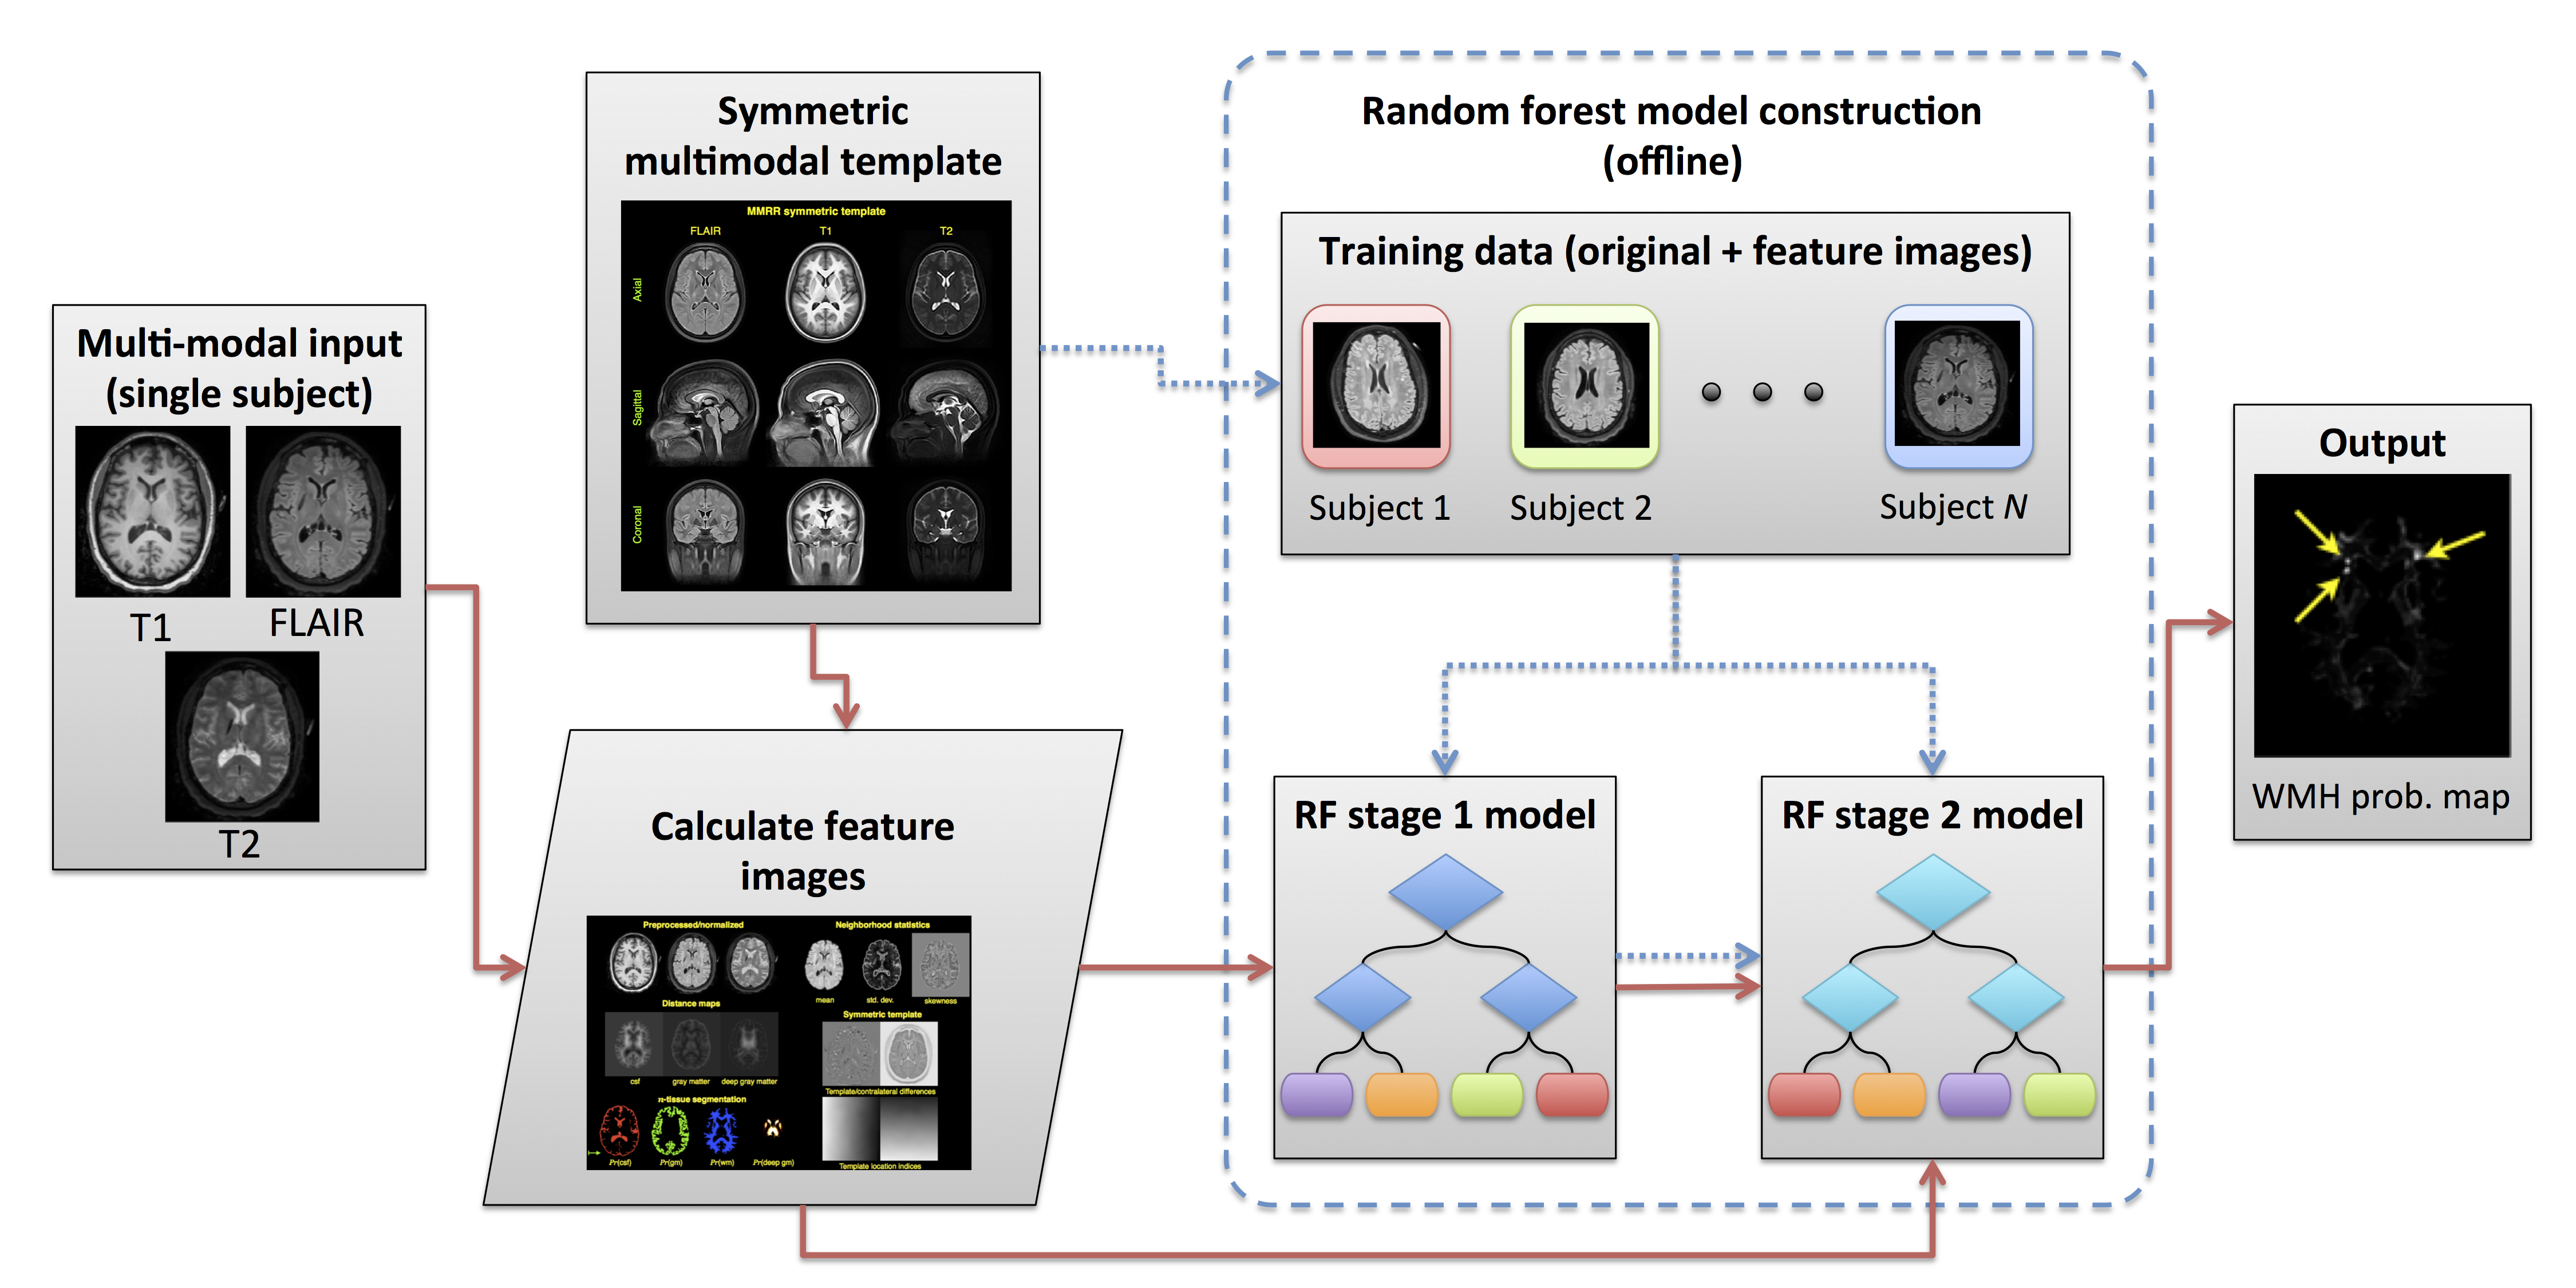
\includegraphics{Figures/wmhPipeline.png}
\caption{\textcolor{blue}{Workflow illustration for the proposed pipeline.  Processing of the multi-modal
input MRI for a single subject, using the multi-modal symmetric template, results in
the generation of the feature images.  These feature images are used as input to the
Stage 1 RF model producing the initial RF probability map estimates.  The Stage 1
voting maps, the original feature images, and the Stage 2 RF model result in the
final voting maps which includes the WMH probability estimate.  Note that the RF models
are constructed once from a set of training data which are processed using the
same feature-construction pipeline as the single-subject input MRI.}}
\end{figure}

\hypertarget{refs}{}

\end{document}
